\chapter{Monte Carlo Simulation}    

The modern version of the Monte Carlo method was invented in the late
1940s by Stanislaw Ulam, while he was working on nuclear weapons
projects at the Los Alamos National Laboratory.
Monte Carlo methods, or Monte Carlo experiments, are a broad class of
computational algorithms that rely on repeated random sampling to obtain
numerical results. 

Monte Carlo simulation is widely used in many fields: engineering,
physics, computational biology, computer graphics, applied statistics,
artificial intelligence for games, search and rescue and of course
finance and business.
In this chapter we will review it and see some useful application to finance.

\section{The algorithm}\label{whats-monte-carlo-simulation}

The underlying concept to Monte Carlo simulation is to use randomness to solve
problems that might be deterministic in principle. These methods
are mainly used in three problem classes: optimization, numerical
integration, and generating draws from a probability distribution.

In principle, Monte Carlo can be used to solve any problem
having a probabilistic interpretation since by the law of large numbers, the
expected value of some random variable ($Y$) can be approximated by taking the
empirical mean of independent samples of the variable:

\[ \hat{\mu}_n = \frac{1}{n}\sum_{i=1}^{n}{Y_i} \]

Monte Carlo methods vary, but tend to follow this particular pattern:
\begin{itemize}
\tightlist
\item
  define a domain of possible inputs;
\item
  generate inputs randomly from a probability distribution over the
  defined domain;
\item
  perform a deterministic computation on the generated inputs;
\item
  aggregate the results.
\end{itemize}
In the next sections we will see each point applied to a practical example.

\section{Pseudo-Random Numbers}\label{pseudo-random-numbers}

Usage of Monte Carlo methods require large amounts of random numbers to
generate the inputs, and it was their use that spurred the development
of pseudo-random number generators. 

Every language has libraries that
allows to produce huge series of random numbers (with a periodicity of
\(2^{19937}\)). Those numbers are produced by algorithms that take as
input a \emph{seed} which determines uniquely the series. This means
that setting the same seed you will produce the same set of numbers
every time (which is great for debugging purposes).

In \texttt{python} the right module to use is \texttt{random} which has the
following useful functions:
\begin{itemize}
\tightlist
\item
  \texttt{seed} set the seed of the random number generator;
\item
  \texttt{random} returns a random number between 0 and 1 (with uniform
  probability);
\item
  \texttt{randint(min,\ max)} returns an integer random number between
  \texttt{min} and \texttt{max} (with uniform probability);
\item
  \texttt{sample(aList,\ k=n)} samples n elements from the list
  \texttt{aList}.
\end{itemize}
As usual for a more detailed description check \texttt{help(random)}. Look at the next example that shows the effect of 
changing the seed of the random number generator.

\begin{tcolorbox}[breakable, size=fbox, boxrule=1pt, pad at break*=1mm,colback=cellbackground, colframe=cellborder]
\begin{Verbatim}[commandchars=\\\{\}]
\PY{k+kn}{import} \PY{n+nn}{random} 

\PY{n}{random}\PY{o}{.}\PY{n}{seed}\PY{p}{(}\PY{l+m+mi}{1}\PY{p}{)}
\PY{n+nb}{print} \PY{p}{(}\PY{l+s+s2}{\PYZdq{}}\PY{l+s+s2}{seed is 1}\PY{l+s+s2}{\PYZdq{}}\PY{p}{)}
\PY{n+nb}{print}\PY{p}{(}\PY{n}{random}\PY{o}{.}\PY{n}{random}\PY{p}{(}\PY{p}{)}\PY{p}{)}
\PY{n+nb}{print}\PY{p}{(}\PY{n}{random}\PY{o}{.}\PY{n}{random}\PY{p}{(}\PY{p}{)}\PY{p}{)}

\PY{n}{random}\PY{o}{.}\PY{n}{seed}\PY{p}{(}\PY{l+m+mi}{2}\PY{p}{)}
\PY{n+nb}{print} \PY{p}{(}\PY{l+s+s2}{\PYZdq{}}\PY{l+s+s2}{seed is 2}\PY{l+s+s2}{\PYZdq{}}\PY{p}{)}
\PY{n+nb}{print}\PY{p}{(}\PY{n}{random}\PY{o}{.}\PY{n}{random}\PY{p}{(}\PY{p}{)}\PY{p}{)}
\PY{n+nb}{print}\PY{p}{(}\PY{n}{random}\PY{o}{.}\PY{n}{random}\PY{p}{(}\PY{p}{)}\PY{p}{)}

\PY{n}{random}\PY{o}{.}\PY{n}{seed}\PY{p}{(}\PY{l+m+mi}{1}\PY{p}{)}
\PY{n+nb}{print} \PY{p}{(}\PY{l+s+s2}{\PYZdq{}}\PY{l+s+s2}{seed is 1 again}\PY{l+s+s2}{\PYZdq{}}\PY{p}{)}
\PY{n+nb}{print}\PY{p}{(}\PY{n}{random}\PY{o}{.}\PY{n}{random}\PY{p}{(}\PY{p}{)}\PY{p}{)}
\PY{n+nb}{print}\PY{p}{(}\PY{n}{random}\PY{o}{.}\PY{n}{random}\PY{p}{(}\PY{p}{)}\PY{p}{)}

\PY{n+nb}{print}\PY{p}{(}\PY{n}{random}\PY{o}{.}\PY{n}{randint}\PY{p}{(}\PY{l+m+mi}{1}\PY{p}{,} \PY{l+m+mi}{10}\PY{p}{)}\PY{p}{)}
\PY{n}{aList} \PY{o}{=} \PY{p}{[}\PY{l+s+s1}{\PYZsq{}}\PY{l+s+s1}{a}\PY{l+s+s1}{\PYZsq{}}\PY{p}{,} \PY{l+s+s1}{\PYZsq{}}\PY{l+s+s1}{b}\PY{l+s+s1}{\PYZsq{}}\PY{p}{,} \PY{l+s+s1}{\PYZsq{}}\PY{l+s+s1}{c}\PY{l+s+s1}{\PYZsq{}}\PY{p}{,} \PY{l+s+s1}{\PYZsq{}}\PY{l+s+s1}{d}\PY{l+s+s1}{\PYZsq{}}\PY{p}{,} \PY{l+s+s1}{\PYZsq{}}\PY{l+s+s1}{f}\PY{l+s+s1}{\PYZsq{}}\PY{p}{]}
\PY{n+nb}{print} \PY{p}{(}\PY{n}{random}\PY{o}{.}\PY{n}{sample}\PY{p}{(}\PY{n}{aList}\PY{p}{,} \PY{n}{k}\PY{o}{=}\PY{l+m+mi}{2}\PY{p}{)}\PY{p}{)}

seed is 1
0.13436424411240122
0.8474337369372327
seed is 2
0.9560342718892494
0.9478274870593494
seed is 1 again
0.13436424411240122
0.8474337369372327
2
['c', 'a']
    \end{Verbatim}
\end{tcolorbox}

Here how it can be drawn a uniform distribution.

 \begin{tcolorbox}[breakable, size=fbox, boxrule=1pt, pad at break*=1mm,colback=cellbackground, colframe=cellborder]
\begin{Verbatim}[commandchars=\\\{\}]
\PY{n}{numbers} \PY{o}{=} \PY{p}{[}\PY{p}{]}
\PY{k}{for} \PY{n}{\PYZus{}} \PY{o+ow}{in} \PY{n+nb}{range}\PY{p}{(}\PY{l+m+mi}{10000}\PY{p}{)}\PY{p}{:}
  \PY{n}{numbers}\PY{o}{.}\PY{n}{append}\PY{p}{(}\PY{n}{random}\PY{o}{.}\PY{n}{randint}\PY{p}{(}\PY{l+m+mi}{0}\PY{p}{,} \PY{l+m+mi}{5}\PY{p}{)}\PY{p}{)}

\PY{k+kn}{from} \PY{n+nn}{matplotlib} \PY{k}{import} \PY{n}{pyplot} \PY{k}{as} \PY{n}{plt}
\PY{n}{plt}\PY{o}{.}\PY{n}{hist}\PY{p}{(}\PY{n}{numbers}\PY{p}{,} \PY{l+m+mi}{6}\PY{p}{,} \PY{n+nb}{range}\PY{o}{=}\PY{p}{[}\PY{o}{\PYZhy{}}\PY{l+m+mf}{0.5}\PY{p}{,} \PY{l+m+mf}{5.5}\PY{p}{]}\PY{p}{)}
\PY{n}{plt}\PY{o}{.}\PY{n}{title}\PY{p}{(}\PY{l+s+s2}{\PYZdq{}}\PY{l+s+s2}{Uniform distribution from randint}\PY{l+s+s2}{\PYZdq{}}\PY{p}{)}
\PY{n}{plt}\PY{o}{.}\PY{n}{show}\PY{p}{(}\PY{p}{)}
\end{Verbatim}
\end{tcolorbox}

\begin{figure}[h]
\centering
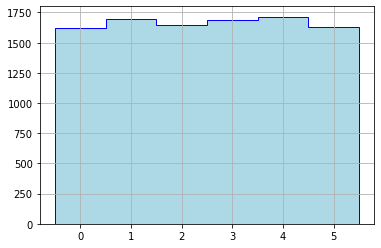
\includegraphics[width=0.7\textwidth]{lecture_6_files/lecture_6_28_0.png}
\end{figure}
Notice the \texttt{\_} following the \texttt{for} statement, it can be used whenever we want to make a loop but we are not interested in the looping variable. 
    
Another useful module that we will use later to generate random numbers is \texttt{numpy}, it has similar functionalities as \texttt{random} but in some cases it fits better to our needs.    
Below an example with \texttt{numpy.random} which allows to throw random numbers according to a normal distribution
(\(\mathcal{N}(0, 1)\)).

 \begin{tcolorbox}[breakable, size=fbox, boxrule=1pt, pad at break*=1mm,colback=cellbackground, colframe=cellborder]
\begin{Verbatim}[commandchars=\\\{\}]
\PY{k+kn}{from} \PY{n+nn}{numpy}\PY{n+nn}{.}\PY{n+nn}{random} \PY{k}{import} \PY{n}{normal}
\PY{k+kn}{from} \PY{n+nn}{matplotlib} \PY{k}{import} \PY{n}{pyplot} \PY{k}{as} \PY{n}{plt}

\PY{n}{gauss} \PY{o}{=} \PY{p}{[}\PY{p}{]}
\PY{k}{for} \PY{n}{\PYZus{}} \PY{o+ow}{in} \PY{n+nb}{range}\PY{p}{(}\PY{l+m+mi}{50000}\PY{p}{)}\PY{p}{:}
  \PY{n}{gauss}\PY{o}{.}\PY{n}{append}\PY{p}{(}\PY{n}{normal}\PY{p}{(}\PY{p}{)}\PY{p}{)}
  
\PY{n}{plt}\PY{o}{.}\PY{n}{hist}\PY{p}{(}\PY{n}{gauss}\PY{p}{,} \PY{l+m+mi}{100}\PY{p}{,} \PY{n+nb}{range}\PY{o}{=}\PY{p}{[}\PY{o}{\PYZhy{}}\PY{l+m+mi}{4}\PY{p}{,} \PY{l+m+mi}{4}\PY{p}{]}\PY{p}{)}
\PY{n}{plt}\PY{o}{.}\PY{n}{title}\PY{p}{(}\PY{l+s+s2}{\PYZdq{}}\PY{l+s+s2}{Example of Gaussian distribution from numpy}\PY{l+s+s2}{\PYZdq{}}\PY{p}{)}
\PY{n}{plt}\PY{o}{.}\PY{n}{show}\PY{p}{(}\PY{p}{)}
\end{Verbatim}
\end{tcolorbox}

    \begin{figure}
    \centering
    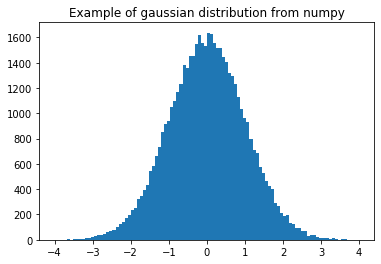
\includegraphics[width=0.7\textwidth]{lecture_6_files/lecture_6_32_0.png}
    \end{figure}

\section{Practical Examples of Monte Carlo
Simulation}\label{example-of-monte-carlo-simulation}

In this section we go through some simple applications of the Monte Carlo method.

\subsubsection{Probability to draw two kings from a deck}
Using a frequentist approach, we can calculate the
probability of an event as the ratio of the number of favorable outcomes
of an experiment (number of successes) and the number of all possible
outcomes. 

Imagine we would like to determine the probability of drawing two kings from a standard deck of cards.
At the beginning we have 40 cards (i.e. the entire deck) with 4 possible kings so the probability to get a king
is $4/40$. Next, assuming we got a king the first time, we are left with 39 cards and 3 kings only so the 
probability to get the second king is $3/39$. Since the two draws are independent, the total probability 
is product of the two contributions, indeed:

\[P_\textrm{two kings} = \frac{4}{40} \cdot \frac{3}{39} = \frac{1}{130} \approx 0.0077\]

Let's now try with a Monte Carlo simulation following the steps outlined above and check if we get the same number.
\begin{itemize}
\item \emph{Define a domain of possible inputs}: in this case the domain is a deck of cards. With the \texttt{*} operator a list can be easily repeated many times. So in this case we do it 4 times, once for each suit (in the example we also set the seed to 1 to make
it reproducible).

\begin{tcolorbox}[breakable, size=fbox, boxrule=1pt, pad at break*=1mm,colback=cellbackground, colframe=cellborder]
\begin{Verbatim}[commandchars=\\\{\}]
\PY{k+kn}{from} \PY{n+nn}{random} \PY{k}{import} \PY{n}{sample}\PY{p}{,} \PY{n}{choices}\PY{p}{,} \PY{n}{seed}

\PY{n}{seed}\PY{p}{(}\PY{l+m+mi}{1}\PY{p}{)}

\PY{n}{deck} \PY{o}{=} \PY{p}{[}\PY{l+s+s2}{\PYZdq{}}\PY{l+s+s2}{A}\PY{l+s+s2}{\PYZdq{}}\PY{p}{,} \PY{l+s+s2}{\PYZdq{}}\PY{l+s+s2}{2}\PY{l+s+s2}{\PYZdq{}}\PY{p}{,} \PY{l+s+s2}{\PYZdq{}}\PY{l+s+s2}{3}\PY{l+s+s2}{\PYZdq{}}\PY{p}{,} \PY{l+s+s2}{\PYZdq{}}\PY{l+s+s2}{4}\PY{l+s+s2}{\PYZdq{}}\PY{p}{,} \PY{l+s+s2}{\PYZdq{}}\PY{l+s+s2}{5}\PY{l+s+s2}{\PYZdq{}}\PY{p}{,} \PY{l+s+s2}{\PYZdq{}}\PY{l+s+s2}{6}\PY{l+s+s2}{\PYZdq{}}\PY{p}{,} \PY{l+s+s2}{\PYZdq{}}\PY{l+s+s2}{7}\PY{l+s+s2}{\PYZdq{}}\PY{p}{,} \PY{l+s+s2}{\PYZdq{}}\PY{l+s+s2}{J}\PY{l+s+s2}{\PYZdq{}}\PY{p}{,} \PY{l+s+s2}{\PYZdq{}}\PY{l+s+s2}{Q}\PY{l+s+s2}{\PYZdq{}}\PY{p}{,} \PY{l+s+s2}{\PYZdq{}}\PY{l+s+s2}{K}\PY{l+s+s2}{\PYZdq{}}\PY{p}{]} \PY{o}{*} \PY{l+m+mi}{4}
 \end{Verbatim}
\end{tcolorbox}

\item \emph{Generate inputs randomly from a probability distribution over the defined domain}: which means we draw randomly cards with uniform probability since the deck is fair and all cards have the same probability to be drawn. 
We plan to do 1 million of simulations (our denominator), each time with the \texttt{sample} function we pick up two cards from our virtual deck with uniform probability. For debugging purpose the first 10 trials are printed.

\begin{tcolorbox}[breakable, size=fbox, boxrule=1pt, pad at break*=1mm,colback=cellbackground, colframe=cellborder]
\begin{Verbatim}[commandchars=\\\{\}]
\PY{n}{trials} \PY{o}{=} \PY{l+m+mi}{1000000}
\PY{n}{success} \PY{o}{=} \PY{l+m+mi}{0}

\PY{k}{for} \PY{n}{i} \PY{o+ow}{in} \PY{n+nb}{range}\PY{p}{(}\PY{n}{trials}\PY{p}{)}\PY{p}{:}
  \PY{n}{cards} \PY{o}{=} \PY{n}{sample}\PY{p}{(}\PY{n}{deck}\PY{p}{,} \PY{n}{k}\PY{o}{=}\PY{l+m+mi}{2}\PY{p}{)}
  \PY{k}{if} \PY{n}{i} \PY{o}{\PYZlt{}} \PY{l+m+mi}{10}\PY{p}{:}
    \PY{n+nb}{print} \PY{p}{(}\PY{n}{cards}\PY{p}{)}
\end{Verbatim}
\end{tcolorbox}

\item \emph{Perform a deterministic computation on the generated inputs}: this step is particularly simple in this case, we just need to check if the draw is \texttt{['K', 'K']} and in case increase the counter of successes.

\begin{tcolorbox}[breakable, size=fbox, boxrule=1pt, pad at break*=1mm,colback=cellbackground, colframe=cellborder]
\begin{Verbatim}[commandchars=\\\{\}]
  \PY{k}{if} \PY{n}{cards} \PY{o}{==} \PY{p}{[}\PY{l+s+s2}{\PYZdq{}}\PY{l+s+s2}{K}\PY{l+s+s2}{\PYZdq{}}\PY{p}{,} \PY{l+s+s2}{\PYZdq{}}\PY{l+s+s2}{K}\PY{l+s+s2}{\PYZdq{}}\PY{p}{]}\PY{p}{:}
    \PY{n}{success} \PY{o}{+}\PY{o}{=} \PY{l+m+mi}{1}
 \end{Verbatim}
\end{tcolorbox}

\item \emph{Aggregate the results}: finally we just print success/trials which is the sought probability.

\begin{tcolorbox}[breakable, size=fbox, boxrule=1pt, pad at break*=1mm,colback=cellbackground, colframe=cellborder]
\begin{Verbatim}[commandchars=\\\{\}]
\PY{n+nb}{print} \PY{p}{(}\PY{l+s+s2}{\PYZdq{}}\PY{l+s+s2}{The probability to draw two kings is }\PY{l+s+si}{\PYZob{}:.4f\PYZcb{}}\PY{l+s+s2}{\PYZdq{}}\PY{o}{.}\PY{n}{format}\PY{p}{(}\PY{n}{success}\PY{o}{/}\PY{n}{trials}\PY{p}{)}\PY{p}{)}

['Q', '7']
['5', '7']
['J', '2']
['Q', 'A']
['5', '4']
['7', '2']
['2', '5']
['J', 'Q']
['A', 'Q']
['J', '5']
The probability to draw two kings is 0.0077
    \end{Verbatim}
\end{tcolorbox}
\end{itemize}

\subsubsection{Dice probabilities}
Two dice are rolled, find the probability that the sum is:
\begin{enumerate}
\item equal to 1
\item equal to 4
\item less than 13
\end{enumerate}

Before looking at the \texttt{python} implementation let's compute what we should get: the possible combinations
of the outcomes of two dice are 36 (to realize it you can simply write them down). It is not possible to get 1 since
thee dice have no face with 0 so the first probability should come out 0. The sum of the two dice is always less than 13 
(the maximum is 12...) so the answer to point 3 is 1. We can get a sum of 4 in 3 cases (1-3, 3-1 or 2-2) so the 
probability will result $3/36=1/12=0.0833$

\begin{tcolorbox}[breakable, size=fbox, boxrule=1pt, pad at break*=1mm,colback=cellbackground, colframe=cellborder]
\begin{Verbatim}[commandchars=\\\{\}]
\PY{k+kn}{import} \PY{n+nn}{random}

\PY{n}{random}\PY{o}{.}\PY{n}{seed}\PY{p}{(}\PY{l+m+mi}{1}\PY{p}{)}

\PY{n}{successes} \PY{o}{=} \PY{p}{\PYZob{}}\PY{l+s+s2}{\PYZdq{}}\PY{l+s+s2}{=0}\PY{l+s+s2}{\PYZdq{}}\PY{p}{:}\PY{l+m+mf}{0.0}\PY{p}{,} \PY{l+s+s2}{\PYZdq{}}\PY{l+s+s2}{=4}\PY{l+s+s2}{\PYZdq{}}\PY{p}{:}\PY{l+m+mf}{0.0}\PY{p}{,} \PY{l+s+s2}{\PYZdq{}}\PY{l+s+s2}{\PYZlt{}13}\PY{l+s+s2}{\PYZdq{}}\PY{p}{:}\PY{l+m+mf}{0.0}\PY{p}{\PYZcb{}}
\PY{n}{trials} \PY{o}{=} \PY{l+m+mi}{100000}
\PY{k}{for} \PY{n}{\PYZus{}} \PY{o+ow}{in} \PY{n+nb}{range}\PY{p}{(}\PY{n}{trials}\PY{p}{)}\PY{p}{:}
    \PY{n}{d1} \PY{o}{=} \PY{n}{random}\PY{o}{.}\PY{n}{randint}\PY{p}{(}\PY{l+m+mi}{1}\PY{p}{,} \PY{l+m+mi}{6}\PY{p}{)}
    \PY{n}{d2} \PY{o}{=} \PY{n}{random}\PY{o}{.}\PY{n}{randint}\PY{p}{(}\PY{l+m+mi}{1}\PY{p}{,} \PY{l+m+mi}{6}\PY{p}{)}
    \PY{k}{if} \PY{p}{(}\PY{n}{d1} \PY{o}{+} \PY{n}{d2}\PY{p}{)} \PY{o}{==} \PY{l+m+mi}{0}\PY{p}{:}
        \PY{n}{successes}\PY{p}{[}\PY{l+s+s2}{\PYZdq{}}\PY{l+s+s2}{=0}\PY{l+s+s2}{\PYZdq{}}\PY{p}{]} \PY{o}{+}\PY{o}{=} \PY{l+m+mf}{1.0}
    \PY{k}{if} \PY{p}{(}\PY{n}{d1} \PY{o}{+} \PY{n}{d2}\PY{p}{)} \PY{o}{==} \PY{l+m+mi}{4}\PY{p}{:}
        \PY{n}{successes}\PY{p}{[}\PY{l+s+s2}{\PYZdq{}}\PY{l+s+s2}{=4}\PY{l+s+s2}{\PYZdq{}}\PY{p}{]} \PY{o}{+}\PY{o}{=} \PY{l+m+mf}{1.0}
    \PY{k}{if} \PY{p}{(}\PY{n}{d1} \PY{o}{+} \PY{n}{d2}\PY{p}{)} \PY{o}{\PYZlt{}} \PY{l+m+mi}{13}\PY{p}{:}
        \PY{n}{successes}\PY{p}{[}\PY{l+s+s2}{\PYZdq{}}\PY{l+s+s2}{\PYZlt{}13}\PY{l+s+s2}{\PYZdq{}}\PY{p}{]} \PY{o}{+}\PY{o}{=} \PY{l+m+mf}{1.0}
    
\PY{k}{for} \PY{n}{k}\PY{p}{,}\PY{n}{v} \PY{o+ow}{in} \PY{n}{successes}\PY{o}{.}\PY{n}{items}\PY{p}{(}\PY{p}{)}\PY{p}{:}
    \PY{n+nb}{print} \PY{p}{(}\PY{l+s+s2}{\PYZdq{}}\PY{l+s+s2}{P(}\PY{l+s+si}{\PYZob{}\PYZcb{}}\PY{l+s+s2}{): }\PY{l+s+si}{\PYZob{}:.3f\PYZcb{}}\PY{l+s+s2}{\PYZdq{}}\PY{o}{.}\PY{n}{format}\PY{p}{(}\PY{n}{k}\PY{p}{,} \PY{n}{v}\PY{o}{/}\PY{n}{trials}\PY{p}{)}\PY{p}{)}

P(=0): 0.000
P(=4): 0.084
P(<13): 1.000
\end{Verbatim}
\end{tcolorbox}

\subsection{Accuracy of Monte Carlo Simulation}

Since we rely on a frequentist approach naively we can say that the lower is the probability we need to estimate the higher has to be the number of simulated trials. This is because to get a reasonable number of "success" so that the uncertainty in the probability is small, we have to try many times. This is apparent playing with the number of trials in the above simulations. 
This is the main reason why, despite its undoubted power, Monte Carlo simulation is not always the best approach to follow.
Many times indeed the simulation of an experiment requires a lot of computing resources (and time) and it may not be practical to embark into a large simulation.

To quantify the error associated to a Monte Carlo estimate remember that our approximation of true value to determine $\hat{\mu}_n$ is itself a random variable (like $Y$) with its mean and variance. From the law of large numbers the mean is:

\[\mathbb{E}(\hat{\mu}_n) = \frac{1}{n}\sum_{i=1}^{n}\mathbb{E}(Y_i)=\mu \]
while its variance is
\[\mathbb{E}((\hat{\mu}_n - \mu)^2)=\frac{\sigma^2}{n}\]
where $\sigma^2 = \mathrm{Var}(Y)$.

While it is obvious that the estimate should get worse with increased variance and better with increased sample size, this equation  gives us the exact rate of exchange. The root mean squared error (RMSE) of $\hat{\mu}_n = \sigma/\sqrt{\mu}$: to get one more decimal digit of accuracy is like asking for an RMSE one tenth as large, and that requires a 100-fold increase in computation. To get three more digits of accuracy requires one million times as much computation. From that it is clear that simple Monte Carlo
computation is poorly suited for problems that must be answered with high precision.

On the other hand if raising $n$ from $n_1$ to $n_2$ only makes our accuracy a little better, then reducing $n$ from $n_2$ to $n_1$ must only make our accuracy a little worse. We might well decide that software that runs slower, reducing $n$ for a given time budget, is worthwhile if it provides some other benefit, such as a more rapid programming.

 \subsection{Derivation of log-normal Stochastic Differential
Equation}\label{derivation-of-log-normal-stochastic-differential-equation}

In this section we try to see how to implement the simulation of the price of a stock with deviate from a steady state as a result of random fluctuations given by the trades. 

Considering a stock with a price \(S_t\) and an expected rate of return \(\mu\); the relative change
in its price during a period \(dt\) can be decomposed in two parts:

\begin{itemize}
\tightlist
\item
  a deterministic part that is the expected return from the stock held
  during the time period \(dt\) and which can be expressed as \(\mu S_tdt\)
\item
  a stochastic part which reflects the random changes of the market
  (e.g.~as a response to external effects such as unexpected news). A
  reasonable assumption is to take this contribution proportional to the
  stock so \(\sigma S_t dB_t\), where \(dB_t\) is a so called random walk process
  equal to \(\mathcal{N}(0,1)\sqrt{t}\).
\end{itemize}
Putting the two contribution together the resulting differential equation is:

\[dS_t = \mu S_tdt + \sigma S_tdB_t\] or
\[\frac{dS_t}{S_t} = d\textrm{log}(S_t) = \mu dt + \sigma dB_t\]

    The solution of this equation can be derived by applying the
It\(\hat{o}\)'s formula which states that for any given function
\(G(S, t)\) where \(S\) satisfies the following stochastic differential
equation \(dS=a\cdot dt +b\cdot dB_t\) it holds:

\[dG=\big(a\frac{\partial G}{\partial S} + \frac{\partial G}{\partial t} + \frac{1}{2}b^2\frac{\partial^2 G}{\partial S^2} \big)dt + b \frac{\partial G}{\partial S}dB\]

Now if we set \(G = \textrm{log}(S_t)\) we can compute the derivatives:

\[\frac{\partial G}{\partial S} = \frac{1}{S_t}\]

\[\frac{\partial G}{\partial t} = 0\]

\[\frac{\partial^2 G}{\partial S^2} = -\frac{1}{S_t^{2}}\]

Substituting back into the previous equation we get:

\[d(\textrm{log} S_t) = \big(\mu S_t \frac{1}{S_t} + \frac{1}{2}\sigma^2 S_t^2 (-\frac{1}{S_t^2})\big)dt + \sigma\epsilon\sqrt{dt}\]

\[d(\textrm{log} S_t) = \textrm{log} (S_t) - \textrm{log} (S_{t-1}) = \textrm{log} \frac{S_t}{S_{t-1}} = \big(\mu - \frac{1}{2}\sigma^2\big)dt + \sigma\epsilon\sqrt{dt}\]

\[S_t = S_{t-1}e^{\big(\mu - \frac{1}{2}\sigma^2\big)dt + \sigma\epsilon\sqrt{dt}}\]

    As can be seen from the following equation:

\[d(\textrm{log} S_t) = \big(\mu - \frac{1}{2}\sigma^2\big)dt + \sigma\epsilon\sqrt{dt}\]
the change in \(\textrm{log} S_t\) has a constant \emph{drift} with respect to time 
\(\mu - \frac{1}{2}\sigma^2\) and a constant variance rate \(\sigma^2\)
(remember that \(\epsilon\) is a normally distributed random variable
\(\mathcal{N}(0,1)\)). So you have a constant plus a Gaussian
distributed variable, therefore \(\textrm{log} S_t\) at some time \(T\)
is normally distributed with:

\[\textrm{log}S_t - \textrm{log}S_0 \approx\mathcal{N}\big[\big(\mu-\frac{\sigma^2}{2}\big)T, \sigma^2 T\big]\]

This equation shows that \(\textrm{log}S_t\) is normally distributed,
but \textbf{a variable whose logarithm is normally distributed is said
to be log-normal}. Hence the model we have just developed implies that
the stock price at time T, given today's price, is log-normally
distributed. One of the nicer property of a log-normal distribution is to be positive defined 
and that's why log-normality is important because we need to \emph{ensure} that a stock price
will never be negative. This result was indeed expected, in fact looking at the initial \(dS\) equation we
had:

\[dS_t = \mu S_tdt + \sigma S_tdB_t\]
which shows that the closer is \(S_t\) to 0 the smaller is the \(dS\)
variation (so it will never go below 0).

In the exercises relative to this chapter you will be asked to simulate the course of a stock price by applying the equation derived before for $S(t)$.

\subsection{Confidence interval}\label{confidence-interval}

By the \href{https://en.wikipedia.org/wiki/Central_limit_theorem}{central limit theorem} we know that 

\[ \hat{\mu}_n = \frac{1}{n}\sum_{i=1}^{n}Y_i\]
is approximately distributed like a normal distribution with mean $\mu$ and variance $\sigma^2 /n$ ($\mathcal{N}(\mu ,\sigma^2 /n)$). Therefore \( \hat{\mu}_n - \mu \) is approximately distributed as 
\[ \hat{\mu}_n - \mu \approx \frac{\sigma}{\sqrt{n}}Z \]
where $Z=\mathcal{N}(0, 1)$ is the standard Gaussian.

This means that given a Monte Carlo experiment the true value $\mu$ will lay in the interval $\hat{\mu}_n \pm  \frac{\sigma}{\sqrt{n}}Z$ around our estimate. 
\begin{figure}[h]
\centering
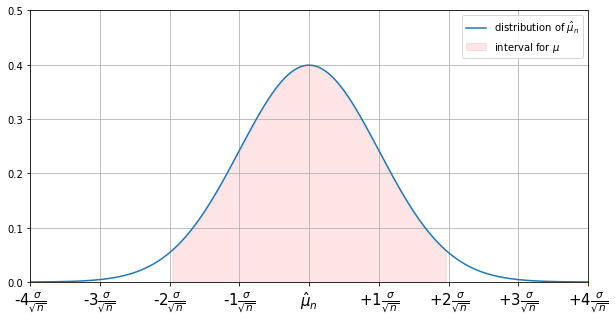
\includegraphics[width=0.7\textwidth]{confidence_interval.png}
\caption{Confidence interval graphical explanation}
\label{fig:confidence}
\end{figure}
Referring to Fig.~\ref{fig:confidence} we can write:
\[\mathbb{P}\Big(\hat{\mu}_n - \frac{1.96\sigma}{\sqrt{n}} \le \mu \le \hat{\mu}_n + \frac{1.96\sigma}{\sqrt{n}}\Big) = 0.95 \]
which corresponds to the shaded area.

The interval above is called 95\% \textbf{confidence interval}. If a variable $X$ is distributed as a Gaussian $\mathcal{N}(\mu, \sigma^2)$ then
\[\mathbb{P}(\mu - 1.96\sigma \le X \le \mu+ 1.96\sigma) = 0.95 \]
because the interval $\pm 1.96\sigma$ covers 95\% of the total area under the Gaussian, in formula $\Phi(1.96)=0.975$ where $\Phi$ is the Gaussian cumulative distribution function.

To construct a confidence interval with a confidence level $\alpha$ different from 0.95, we have to find a number $A$ such that 
\[\Phi(A) = 1 - \frac{1-\alpha}{2}\]
then the $\alpha$-confidence interval
\[\mathbb{P}(\mu - A\sigma \le X \le \mu+ A\sigma) = \alpha \]

The width of the confidence interval is a measure of the accuracy of our estimate.
$\alpha$-confidence interval can be expressed in terms of repeated
experiments like the following: if you repeat many time the above simulation,
the fraction of calculated confidence intervals (which would differ for each sample) that contains
the true parameter would tend toward $\alpha \%$ (beware! in $1-\alpha\%$ of cases it is outside the interval!).

The width of the confidence interval depends on two factors: number of simulations $n$ and variance of the variable $\sigma$.
The size of the confidence interval shrinks like the inverse square root of the number of samples. This is
one of the main disadvantages of Monte Carlo method.

Below an example of how to compute a confidence level in \texttt{python} given a set of fake simulations:

\begin{tcolorbox}[breakable, size=fbox, boxrule=1pt, pad at break*=1mm,colback=cellbackground, colframe=cellborder]
\begin{Verbatim}[commandchars=\\\{\}]
\PY{k+kn}{import} \PY{n+nn}{numpy} \PY{k}{as} \PY{n+nn}{np}
\PY{k+kn}{from} \PY{n+nn}{scipy}\PY{n+nn}{.}\PY{n+nn}{stats} \PY{k}{import} \PY{n}{norm}

\PY{n}{samples} \PY{o}{=} \PY{p}{[}\PY{l+m+mf}{1.}\PY{p}{,}\PY{l+m+mf}{2.}\PY{p}{,}\PY{l+m+mf}{3.}\PY{p}{,}\PY{l+m+mf}{4.}\PY{p}{,}\PY{l+m+mf}{4.}\PY{p}{,}\PY{l+m+mf}{4.}\PY{p}{,}\PY{l+m+mf}{5.}\PY{p}{,}\PY{l+m+mf}{5.}\PY{p}{,}\PY{l+m+mf}{5.}\PY{p}{,}\PY{l+m+mf}{5.}\PY{p}{,}\PY{l+m+mf}{4.}\PY{p}{,}\PY{l+m+mf}{4.}\PY{p}{,}\PY{l+m+mf}{4.}\PY{p}{,}\PY{l+m+mf}{6.}\PY{p}{,}\PY{l+m+mf}{7.}\PY{p}{,}\PY{l+m+mf}{8.}\PY{p}{]}
\PY{n}{alpha} \PY{o}{=} \PY{l+m+mf}{0.95}

\PY{n}{X} \PY{o}{=} \PY{n}{np}\PY{o}{.}\PY{n}{array}\PY{p}{(}\PY{n}{samples}\PY{p}{)}
\PY{n}{A} \PY{o}{=} \PY{n}{norm}\PY{o}{.}\PY{n}{ppf}\PY{p}{(}\PY{p}{(}\PY{l+m+mi}{1} \PY{o}{+} \PY{n}{alpha}\PY{p}{)}\PY{o}{/}\PY{l+m+mi}{2}\PY{p}{)}
\PY{n}{m}\PY{p}{,} \PY{n}{se} \PY{o}{=} \PY{n}{np}\PY{o}{.}\PY{n}{mean}\PY{p}{(}\PY{n}{X}\PY{p}{)}\PY{p}{,} \PY{n}{np}\PY{o}{.}\PY{n}{std}\PY{p}{(}\PY{n}{X}\PY{p}{)}
\PY{n}{h} \PY{o}{=} \PY{n}{A}\PY{o}{*}\PY{n}{se}\PY{o}{/}\PY{n}{np}\PY{o}{.}\PY{n}{sqrt}\PY{p}{(}\PY{n+nb}{len}\PY{p}{(}\PY{n}{samples}\PY{p}{)}\PY{p}{)}
\PY{n+nb}{print} \PY{p}{(}\PY{l+s+s2}{\PYZdq{}}\PY{l+s+si}{\PYZob{}:.0f\PYZcb{}}\PY{l+s+si}{\PYZpc{} c}\PY{l+s+s2}{onfidence interval: }\PY{l+s+si}{\PYZob{}\PYZcb{}}\PY{l+s+s2}{ +\PYZhy{} }\PY{l+s+si}{\PYZob{}\PYZcb{}}\PY{l+s+s2}{\PYZdq{}}\PY{o}{.}\PY{n}{format}\PY{p}{(}\PY{n}{alpha}\PY{o}{*}\PY{l+m+mi}{100}\PY{p}{,} \PY{n}{m}\PY{p}{,} \PY{n}{h}\PY{p}{)}\PY{p}{)}

95\% confidence interval: 4.4375 +- 0.8119808363806419
\end{Verbatim}
\end{tcolorbox}
